%格式設定%
\documentclass[a4paper,12pt]{article}
\usepackage[utf8]{inputenc}
\usepackage{xeCJK}
\usepackage{fontspec}
\usepackage{graphicx}
\setmainfont{Times New Roman}
\setCJKmainfont{kaiu.ttf}

\title{日麻講義}
\author{Esean}

\begin{document}
\maketitle

\tableofcontents

\part{基本}
\section{滿貫以下的算點}
自己算點是從網麻到實麻的第一步。為了估計要和多少才能逆轉，學會自己算點不論是在網麻抑或實麻都是十分重要的。
\subsection{符數計算}
它簡單來說就是100以內的加法，應該不難吧(笑) \\
首先，我們有底符20，接著看看自己的手牌構成:把所有順子刪掉只看刻子和雀頭。以中張明刻為基準2符，暗刻乘2，明槓再乘2，暗槓再乘2。么九牌的符數是中張的兩倍。
整理成表格如下: \\
\begin{tabular}[t]{l|llll}
\ & 明刻 & 暗刻 & 明槓 & 暗槓 \\
\hline\hline
中張 & 2 & 4 & 8 & 16 \\
么九 & 4 & 8 & 16 & 32 \\
\end{tabular}
\\
然後符合的全部加上去。接著是雀頭:役牌2符，連風牌4符(視規則而定)。最後的結果無條件進位到十位就是最後的符數。
\subsection{基本點公式}
把符數做以下運算:$符數 \times 2^{飜數+1}$，這就是基本點，接著參照以下表格: \\
\begin{tabular}[t]{l|ll}
\ & 子家 & 親家 \\
\hline
榮和 & 基本點 $\times 4$ & 基本點 $\times 6$ \\
\hline
自摸和 & 親:基本點 $\times 2$ & 三家各基本點 $\times 2$ \\
\ & 子:基本點 $\times 2$ \\
\end{tabular}
\\
為了避免每次都要用基本點公式硬算，我們有以下速查表: \\
\begin{figure}
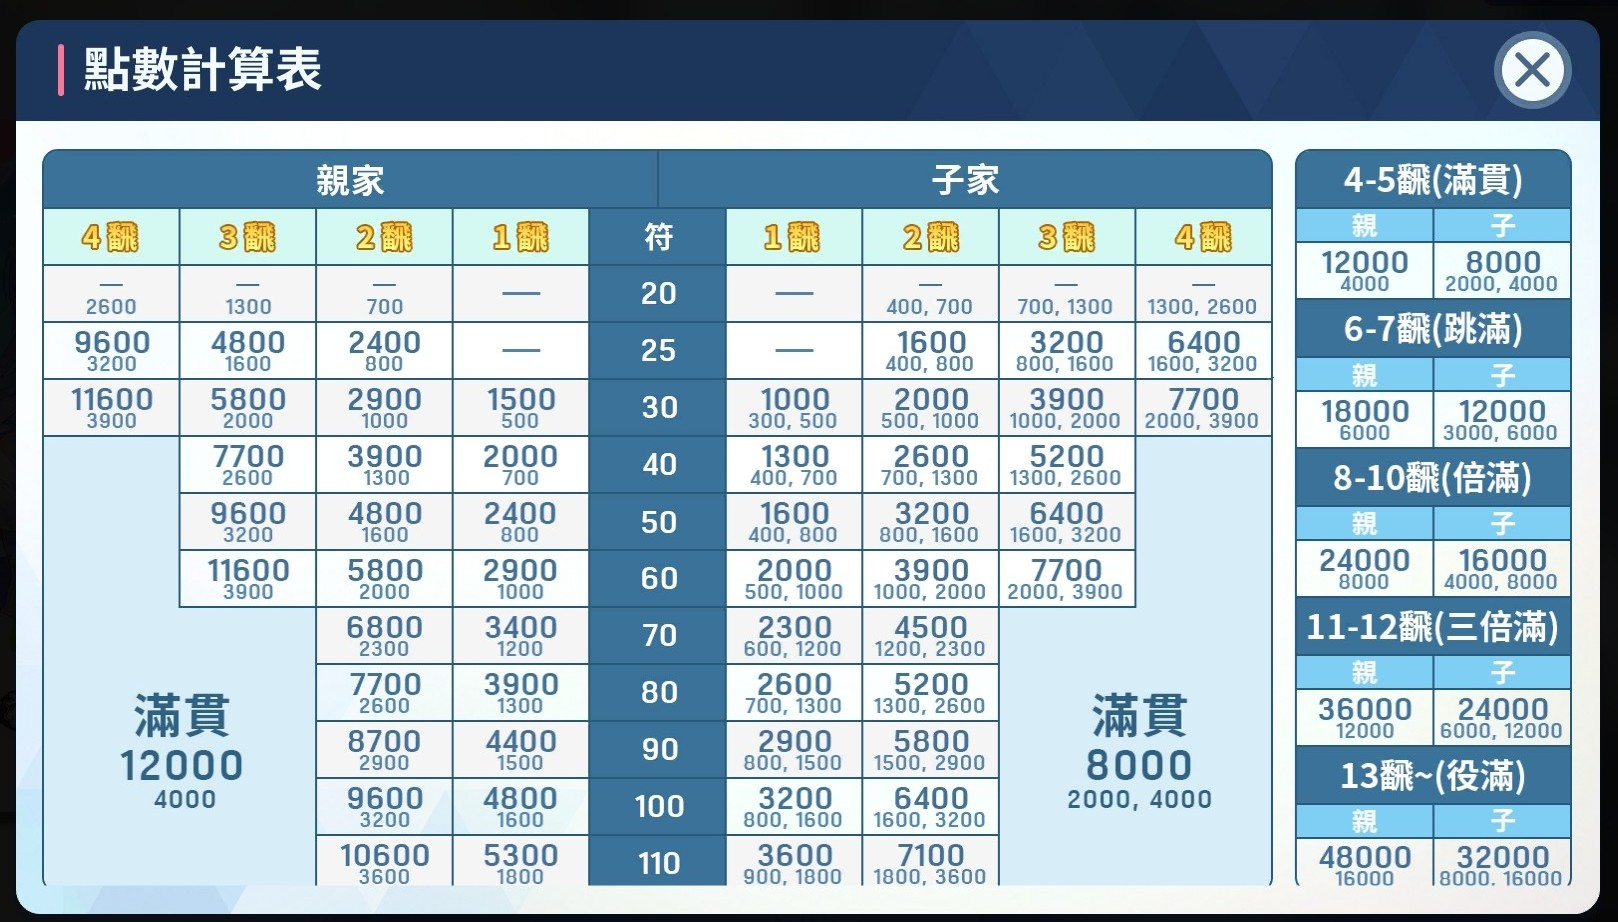
\includegraphics[width=0.8\textwidth]{點數速查表.jpg}
\end{figure}
\section{牌桌禮儀}

\part{基礎牌效率}
\section{前言}
\section{單張牌效率}
\section{對子及三張複合搭}
\section{進階複合搭}
\section{五搭理論}
\section{一向聽集中理論}
\section{有效牌重複理論}

\part{基礎防守理論}
\section{前言}
\section{現物}
\section{筋牌}
\section{壁牌}

\part{鳴牌}
\section{役牌}
\section{斷么}

\part{基礎攻守判斷}

\part{名詞索引}
\end{document}